\documentclass{report}
% Comment the following line to NOT allow the usage of umlauts
\usepackage[utf8]{inputenc}
\usepackage[francais]{babel}
\usepackage{listings}
\usepackage{xcolor}
\usepackage{textcomp}
\usepackage{graphicx}
\usepackage{caption}
\usepackage{chngpage}
\pagestyle{plain}
\definecolor{listinggray}{gray}{0.9}
\definecolor{lbcolor}{rgb}{0.9,0.9,0.9}
\lstset{
backgroundcolor=\color{lbcolor},
tabsize=4,
rulecolor=,
language=matlab,
basicstyle=\scriptsize,
upquote=true,
aboveskip={1.5\baselineskip},
columns=fixed,
showstringspaces=false,
extendedchars=true,
breaklines=true,
prebreak = \raisebox{0ex}[0ex][0ex]{\ensuremath{\hookleftarrow}},
frame=single,
showtabs=false,
showspaces=false,
showstringspaces=false,
identifierstyle=\ttfamily,
keywordstyle=\color[rgb]{0,0,1},
commentstyle=\color[rgb]{0.133,0.545,0.133},
stringstyle=\color[rgb]{0.627,0.126,0.941},
}

\title{Rapport de TER}
% Start the document
\begin{document}
\maketitle
\newpage
\tableofcontents
\newpage
% Create a new 1st level heading

\part{Présentation du projet}
\chapter{Introduction}
\section{But du projet}
\paragraph{}
L'objectif de ce projet est la réalisation d'un jeu basé sur un modèle multi-agent. L'idée générale du projet est dans la continuité du projet de l'année dernière sur le même thème. L'outil utilisé est Unity 3D, un moteur de jeu utilisé dans un grand nombre de réalisations de hautes qualités. Notre projet est utilisable sur Windows et Mac et pourrait être porté sur Android.
Ce projet consiste de réaliser un jeu que l'on peut qualifier de programmeur et de permettre, notamment, à de jeunes personnes de se familiariser avec le monde de la programmation. L'utilisateur pourra donc créer un comportement pour des robots appelé "unité" afin de remplir des objectifs du jeu.
\paragraph{}
Le projet Metabot est un projet modeste réalisé à partir du logiciel Unity 3D par un groupe d'étudiant débutant dans l'utilisation de cet outil. Malgré le peu d'expérience dans la création pure de ce genre de projet, le projet actuel est le fruit d'un travail important et d'une implication entière de toute l'équipe.
Le projet a donc pour unique prétention de communiquer notre amour du jeu vidéo et de la programmation.
Même si les deux équipes étaient séparés sur le papier dans le TER , une étant chargée de reprendre le projet WarBot et le rendre plus générique pour le futur, et l’autre chargée de mettre à jour et rajouter des fonctionnalités au jeu , les 2 équipes ont tout naturellement fusionnée, puisque l’ajout de fonctionnalités n’est possible que lorsque le jeu est terminé , ou assez fonctionnel
\subsection{Cahier des charges}
\section{Notion d'agent}
\subsection{Système multi-agents}
- Agents peu intelligent tel quel , mais c’est la coordination de ces agents qui va construire une “société” intelligente et fonctionnelle
-2  types d’agents : agent cognitif et agent reactif
- Au sein des agents cognitifs , on peut faire une distinction entre des agents ayant un but et des agents ‘support’ qui servent pour donner des informations sur l’univers ax agents avec but
- agents peuvent s’organiser en sociétés , mais aussi plus précisèment en équipe ou en coalitions
\subsection{Langage et communications entre agents}
-Importance de la communications entre agents
-Possible de mettre en place une équipe sans communication dans warbot mais interet extremement limité et victoire quasi impossible face a une equipe organisée
-Certaines unités ne peuvent s’exprimer correctement sans la communication (Rocket Launcher peuvent tirer plus loin que leur perception
- Différentes structures pour définir le comportement des unités dans le cas d’un systeme multi agent (subsumption , FSM , ..) mais on va favoriser l’architecture de sumpsumption car plus simple a comprendre pour les utilisateurs , projet destiné a faire apprendre la programmation
-
\subsection{Representation dans notre projet}
\subsection{Ancient projet}
\newpage
\chapter{WarBot: Le mode par défaut}
\section{Principe}
Dans WarBot, deux à quatre équipes se battent sur un terrain pour les ressources afin de survivre et d'éliminer les autres équipes afin d’être la dernière ne vie. Des ressources apparaissent sur la carte et peuvent etre converti en unité ou en soin.

\newpage
\part{Réalisation du projet}
\newpage


\newpage
\chapter{Partie "Interpreteur"}
repasser sur le texte pour ajouter exemples et illustrations !
\section{Présentation et Attente}
La partie "Interpréteur" est la partie la moins visible du projet MetaBot,
mais il s'agit de la partie du projet servant de clé de voute du jeu.
Comme dit plus tôt, la particularité de MetaBot est que le joueur, qui pourra être considéré comme le programmeur, va préparer en amont une cohésion d'équipe à travers le comportement et va pouvoir lancer un match contre une autre équipe, afin d'évaluer quel comportement sera le meilleur.
L'interpreteur permet de faire la liaison entre l'éditeur du comportement ou l'utilisateur va développer son comportement, en utilisant un ensemble de d'instructions que nous avons prédéfinies  et la partie moteur, ou le fonctionnement des unités est inscrit, ainsi que les différents modes de jeux.
\paragraph{}
Le langage et l'ensemble des instructions nécessaires est alimenté par l'équipe Game Design qui nous a donné des exemples de messages ou de spécificités du langage qui pourrait être nécessaire. On pouvait ensuite tous en discuter en pesant le pour et le contre, afin de définir si la fonctionnalité allait être mise en place , et de quelle façon.
\section{Etude de l'ancien projet et récupération de ce qui est utile}
Au départ, il a été nécessaire de remettre en place un outil permettant de récupérer un comportement, qui était uniquement graphique, dans l'éditeur afin de pouvoir le renvoyer à la partie Moteur, pour que l'ensemble des unités puissent l'exécuter.
Nous avons pris connaissance de ce que l'ancien groupe avait mis en place et avons trié ce qui nous semblait correspondre à notre version du projet.
Il était obligatoire d'écrire le comportement récupéré de l'éditeur dans un fichier, afin de le récupérer , pouvoir le modifier , le déplacer , et le conserver pour plusieurs parties.
La solution mise en place par l'ancien groupe pour le stockage, qui était d'utiliser un fichier XML correspondait parfaitement à notre besoin, car la syntaxe et l'organisation en nœuds de ce genre de fichiers, permettait une récupération simple et claire des instructions. Nous avons ainsi pu récupérer une bonne partie de leur système d'écriture et de lecture de leur projet, tout en adaptant l'autre partie à nos besoins.
\paragraph{}
\newpage
La partie organisant les instructions à été complètement supprimée, et nous avons repensé un système plus générique et plus compréhensible pour les groupes qui vont récupérer ce projet plus tard.
\section{Conception et implémentation}
La construction des Instructions des unités dans la partie Interpréteur a grandement été facilitée et la liaison des instructions avec leur exécution a été décalée dans le moteur. Ainsi on ne manipule que des chaînes de caractères lors de l'accès dans le fichier, et le moteur effectue la liaison avec une structure de "Delegate" comme expliqué plus haut, rajoutant beaucoup de généricité au projet.
D'un point de vue de la sécurité, celle-ci a été décalée dans l'éditeur du comportement, afin de ne pas traiter des comportements erronés , mais prévenir a l'avance et même empêcher les erreurs d'apparaitre.
\paragraph{}
Le but de l'interpréteur était de traiter des fichiers de ce type :
\begin{lstlisting}[frame=single]
<behavior>
 <teamName> Default Team</teamName>
 <unit name="Explorer">
   <instruction>
   </instruction>
 </unit>
 <unit name="Base">
 </unit>
 <unit name="Light">
 </unit>
 <unit name="Heavy">
 </unit>
</behavior>
\end{lstlisting}
Ainsi nous avons 1 fichier par équipe écrite par l'utilisateur, chacun détaillant le comportement de chaque unité sous la même forme :
\begin{lstlisting}[frame=single]
<behavior>
 <teamName> Default Team</teamName>
 <unit name="Explorer">
<instruction>
     <parameters>
       <PERCEPT_ENEMY />
     </parameters>
     <message>
       <ACTN_MESSAGE_HELP>
         <Light />
       </ACTN_MESSAGE_HELP>
     </message>
     <actions>
       <ACTION_MOVE />
     </actions>
   </instruction>
   <instruction>
     <parameters>
       <PERCEPT_BLOCKED />
     </parameters>
     <actions>
       <ACTION_MOVE_UNTIL_UNBLOCKED />
     </actions>
   </instruction>
 </unit>
</behavior>
\end{lstlisting}
Le comportement d'une unité est une suite d'instructions, dont l'ordre est très important. La hiérarchie va déterminer la priorité qu'aura l'action sur le tick. Ainsi l'action la plus prioritaire dont les conditions sont acceptées sera l'action effectuée sur ce tick.
Chaque instruction est toujours organisée de la même façon :
- Une liste de conditions à remplir pour que l'instruction soit considéré comme acceptée
- Une liste d'actions qui ne terminent pas l'action, appelées Actions non terminales, mais qui peuvent être les messages partagés entre les unités par exemple. Ces actions non terminales seront exécutés avant :
- L'action terminale, qui va être exécutée à la fin du tick pour l'ensemble des unités et va être l'action qui va être "physiquement" fait par l'unité, par exemple : Avancer, Tirer, Récupérer ou donner une ressource,Se soigner , ...
\paragraph{}
Comme dit précédemment, l'interpréteur relie les 2 parties majeures du projet.
Ainsi, une fonction permet de transformer un fichier ".wbt" (format des équipes WarBot) vers un comportement d'équipe utilisable par l'équipe moteur, et une fonction permettant la transformation d'un comportement récupéré de l'éditeur graphique vers un fichier XML, pour sa sauvegarde.
\newpage
\paragraph{}
Un nouveau travail d'interprétation a vite été ressenti dans le projet. En effet, le jeu étant destiné à aider les jeunes à appréhender la programmation, une traduction française était nécessaire.
Toujours dans l'idée de rester générique, un traducteur a été mis en place et attaché à l'ensemble des textes qui seront affichés à l'utilisateur.
\paragraph{}
//pas clair a changer
La traduction fonctionne ainsi :
Un premier script s'occupe de vérifier la langue qui doit être utilisée dans le fichier de configuration du jeu et va charger en mémoire un fichier  de traductions :

Le fichier va être parcouru, et un ensemble de couples clé,valeurs vont être récupérés , la clé correspondant à la valeur initiale d'un bouton/ texte affiché, la valeur étant la traduction qu'il faudra affiché à la place de la clé.

Ce script est ainsi rattaché au "GameManager" , un objet Unity qui n'est pas détruit lorsque l'on change de scène. Ainsi les traductions sont conservées lorsqu'on passe de l'éditeur au menu principal , du menu principal aux cartes de jeu, ...
\paragraph{}
Un second script est lui attaché à tous les Objets du jeu qui vont devoir être traduits. Celui-ci va , à la création de l'objet auquel il est rattaché, chercher la langue actuellement affichée, récupérer comme clé le texte original de l'objet auquel le script est affilié, et va stocker la traduction, et l'afficher à l utilisateur.

En Runtime, si la langue est changée dans les paramètres du jeu, les script de traduction des objets vont mettre à jour leur langue, et récupérer la nouvelle traduction dans le "GameManager".

\paragraph{}
La traduction est aussi disponible sans rattacher un script "Traducteur" à un Objet de la scène.
En effet, il y a beaucoup de situations ou on ne peut pas rattacher ce script. On peut récupérer la traduction via le champ "traduction" du traducteur après l'avoir instancié dans un script externe, et l'afficher ou l'utiliser à la place de ce qu'on l'on voulait traduire.
\paragraph{}
La récupération de la langue du projet se fait à travers un fichier paramètre à la création du Traducteur, que ce soit dans la scène ou dans un script.
Celle-ci est stockée en clair dans un fichier de paramétrage :
\paragraph{}
\begin{center}
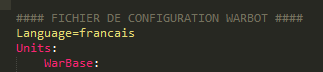
\includegraphics[scale=0.9]{DATA/fichierconfig.png}
\captionof{figure} {Fichier configuration}
\end{center}
\paragraph{}
Mais ce fichier est caché, à moins de connaître sa position dans la hiérarchie et de devoir redémarrer le jeu pour changer la langue, 2 boutons sont dans les paramètres pour passer en Français ou en Anglais. Si le besoin de nouvelles langues se fait sentir dans le futur, il sera toujours possible de transformer ces boutons en un "DropDown" , un menu déroulant, afin de pouvoir sélectionner autant de langues que disponible.
\paragraph{}
L'ajout de traductions est externe au jeu.
Dans les fichiers du jeu , on retrouve un dossier contenant ces traductions,sous formes de fichier représentant chacun une langue.
Une traduction est simplement une ligne du fichier mettant en relation une clé et sa traduction.
Le rajout d'une langue est simple est totalement simple et générique :
On ajoute un fichier ayant le nom de la langue que l'on souhaite, et qui doit obligatoirement implémenter l'ensemble des clés présentes dans les autres fichiers, ou dans le fichier "example" mis à disposition.

Voici à quoi ressemble les fichiers de traduction :
\begin{lstlisting}[frame=single]
# Percepts
    PERCEPT\ALLY=PERCEPT\ALLIE\A\PORTEE
    FALSE\PERCEPT\ALLY=PERCEPT\AUCUN\ALLIE\A\PORTEE
    PERCEPT\BLOCKED=PERCEPT\EST\BLOQUE
    FALSE\PERCEPT\BLOCKED=PERCEPT\N'EST\PAS\BLOQUE
    PERCEPT\IS\RELOADED=PERCEPT\EST\RECHARGE
    FALSE\PERCEPT\IS\RELOADED=PERCEPT\N'EST\PAS\RECHARGE
    PERCEPT\IS\NOT\RELOADED=PERCEPT\PAS\RECHARGE
    FALSE\PERCEPT\IS\NOT\RELOADED=PERCEPT\EST\RECHARGE
# Map en jeu
    Recommencer=Recommencer
    Quitter=Quitter
    Health : =Vie :
    Bag : =Sac :
    Heading : =Orientation :
    Contract :=Contrat :
\end{lstlisting}
On a donc ici bien le système de clé / valeur expliqué plus haut.
On peut voir que le caractère séparateur est le caractère ' = ' , au départ nous utilisions le caractère ' : ' , mais il y a eu des conflits puisque les textes affichés sur l'interface utilisateur contiennent aussi les ':'.
Il est possible que le caractère ' = ' pose problème au bout d'un moment, si jamais des traductions ajoutées ultérieurement le contiennent. Il faudra donc simplement faire une recherche "Trouver et Remplacer" dans les fichiers de traduction, et changer un seul caractère dans le code du Parser des fichiers de traductions.

\paragraph{}

La traduction dupliquée de chaque texte comme vue dans la partie "Percepts" de l'exemple plus haut à laquelle on rajoute un "FALSE\" provient du fait que les conditions et perceptions qui sont traitées dans le jeu peuvent être mises au négatif. Par exemple, si le comportement d'une unité de mon équipe cherche à savoir si cette unité à "un contrat d'élimination en cours" lorsqu'elle reçoit le message demandant de l'aide depuis la base, il est tout à fait possible que l'on cherche à vérifier que l'on a aucun contrat d'élimination pour pouvoir en accepter un nouveau.
Au lieu de dupliquer les conditions dans le code , il a été préféré de pouvoir les rendre négatives.

\newpage
\chapter{Partie "Game Design"}
\section{Expérience utilisateur}
\subsection{Ancienne version de Warbot}
\paragraph{}
    Les premières semaines de ce projet ont été l’occasion pour toute l’équipe de se familiariser avec la version de WarBot qui avait été créé par les étudiants de l’année précédente. Nous avons donc immédiatement essayé de créer des équipes pour tenter d’apprivoiser son éditeur de comportement.
\paragraph{}
\begin{adjustwidth}{-3em}{}
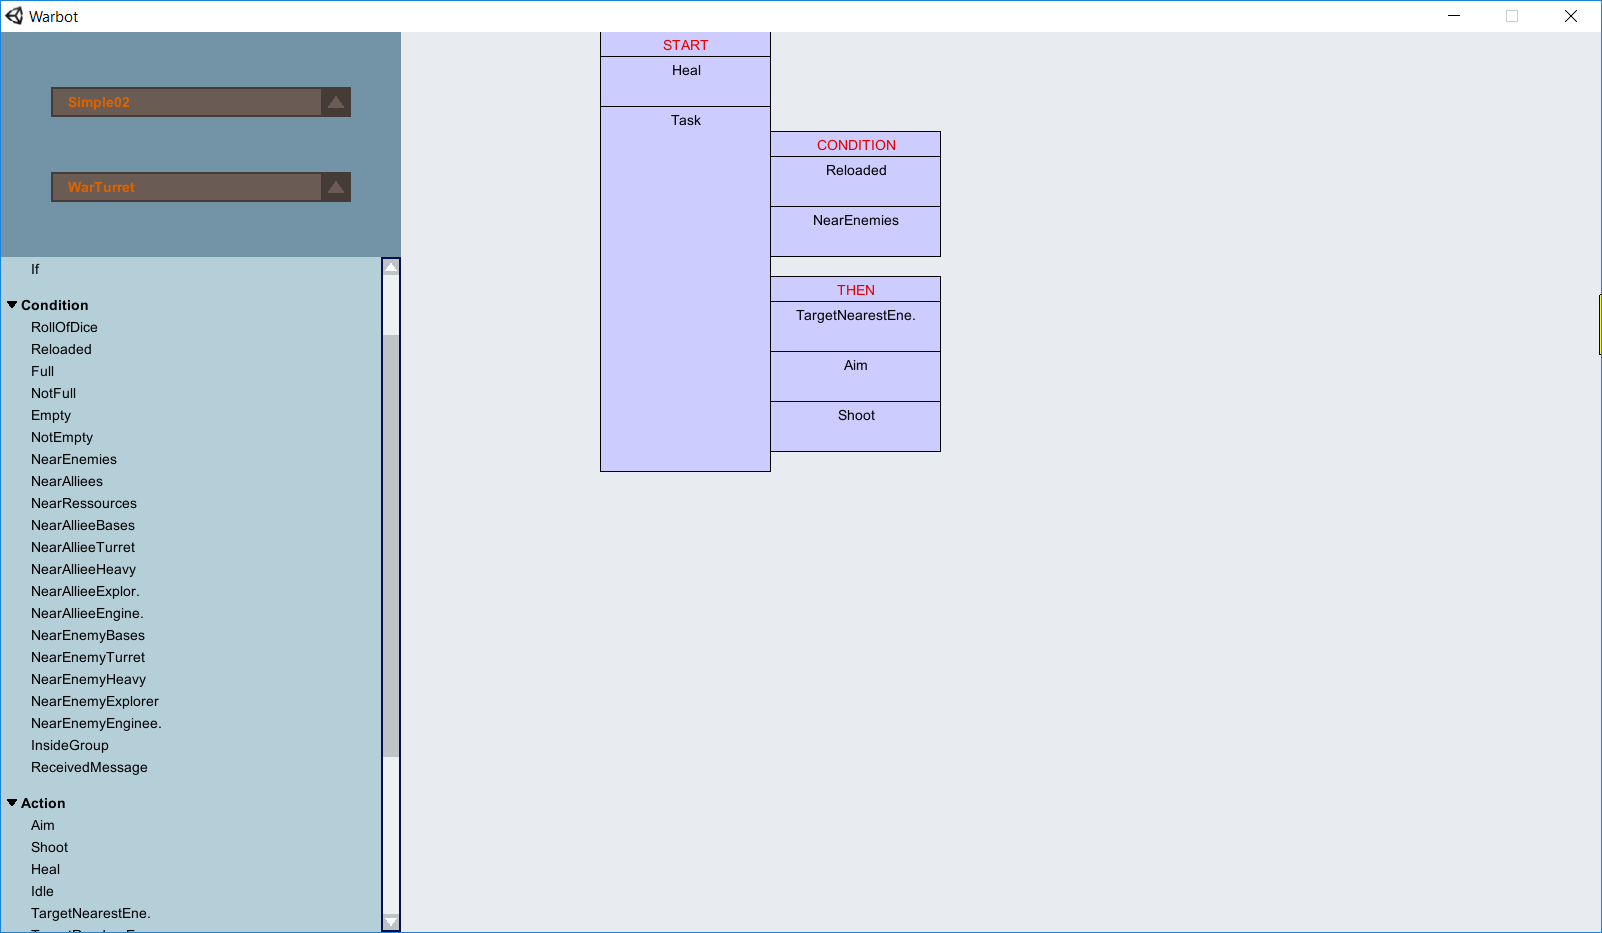
\includegraphics[scale=0.4]{DATA/oldEditor.png}
\captionof{figure} {Aperçu de l'éditeur}
\end{adjustwidth}
\paragraph{}
    Nous nous sommes très vite rendu compte de plusieurs problèmes d’ergonomie qui rendait la création d’équipe difficile.
Tout d’abord, pour placer un bloc, il fallait :
\begin{itemize}
\item Cliquer sur le nom d’une primitive dans le menu de gauche
\item Maintenir le clic de la souris et déplacer le pointeur de la souris sur un bloc déjà placé
\item Le bloc est ensuite placé en-dessous du bloc où se trouve le pointeur de la souris
\end{itemize}
Si cela semble simple sur le papier, en pratique c’est une tout autre histoire car le moindre faux mouvement positionnait le bloc au mauvais endroit ou le faisait disparaître.
En effet, si le curseur de la souris ne se trouvait sur aucun bloc au moment où on relâchait le clic, le bloc était tout simplement supprimé. \newline
Dans le cas où l’on avait mal positionné le bloc il fallait alors le déplacer. Cependant, cliquer sur un bloc déjà existant pour le déplacer entraînait également le déplacement des blocs situés en-dessous de celui que l’on souhaitait déplacer. Il fallait donc, dans un premier temps, sélectionner les blocs en-dessous de la primitive mal placée pour les positionner au-dessus de cette dernière pour pouvoir déplacer la primitive mal placée sans modifier le reste du comportement.
\paragraph{}
    Supprimer un bloc s’il n’est attaché à aucun autre bloc semble être une bonne idée car cette technique permet de ne pas avoir trop de blocs inutiles qui traînent dans l’interface. Seulement, un simple clic sur une primitive supprimait cette dernière ainsi que toutes celles placées en dessous de la primitive supprimé. Ceci s’explique par le fait que lors du clic sur une primitive, l’éditeur estime que nous somme en train de la déplacer. Or, comme on relâche la souris sans la bouger cette dernière est déplacé à un endroit où il n’y a aucun bloc entraînant ainsi sa suppression. \newline
Ce problème était particulièrement dérangeant lorsque l’on souhaitait utiliser WarBot avec un pavé tactile car une simple pression sur ce dernier est compté comme un clic, il n’était pas rare de supprimer une grosse partie de notre comportement en voulant repositionner son doigt sur le pavé tactile.
\paragraph{}
    A ceci s’ajoute l’absence de certaines fonctionnalité comme la possibilité d’annuler une modification ou de choisir quand sauvegarder le fichier, ce qui implique que chaque erreur était sauvegardé et la seule manière de la corriger était de replacer de nouveaux blocs pour revenir au comportement voulu.
\paragraph{}
    Cette version de WarBot possédait plusieurs types de primitives : les primitives de contrôle if et task, les conditions et les actions. Parmis les actions, certaines terminaient le tour de l’unité (tirer, bouger, se soigner…) alors que d’autres permettaient à l’unité de continuer son tour (Rejoindre un groupe, changer l’orientation de l’unité…). Il était difficile de savoir lesquelles terminent le tour ou non car il n’y avait aucune différence visuelle entre ces deux types de primitives. Le seul moyen de savoir si une primitive permettait de continuer son tour était donc de passer sa souris sur le nom d’une primitive dans le menu à gauche pour avoir une description de la primitive dans laquelle il était précisé si cette action terminait le tour de l’unité. Dans le cas où l’action n’était pas terminale, aucune précision n’était rajouté.
\paragraph{}
\begin{center}
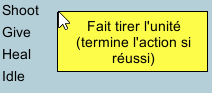
\includegraphics[scale=1]{DATA/terminale1.png}
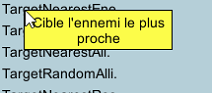
\includegraphics[scale=1]{DATA/terminale2.png}
\captionof{figure} {Comparaison descriptions}
\end{center}
\paragraph{}
    Un dernier problème d’ergonomie important est l’emplacement des boutons dans cet éditeur. En effet, il était possible de revenir au menu principal, de créer une nouvelle partie, de quitter le jeu et de créer une nouvelle équipe depuis l’éditeur. Cependant, les boutons qui permettaient ces actions étaient cachés dans le menu pause de l’éditeur. Le simple fait de pouvoir mettre en pause en écran qui n’en a pas besoin est déjà suffisamment contre-intuitive pour privilégier le fait de placer des boutons directement dans l’interface de l’éditeur plutôt que dans un menu accessible uniquement via la pression de la touche échap du clavier.
\paragraph{}
\begin{center}
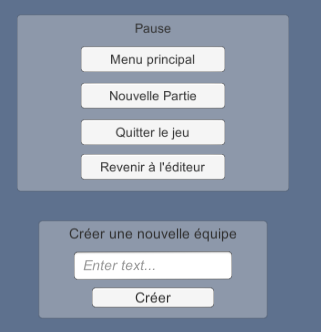
\includegraphics[scale=1]{DATA/oldPause.png}
\captionof{figure} {Fichier configuration}
\end{center}
\paragraph{}

\subsection{Création d’équipe sous la version actuelle}
\section{Test logiciel}
\subsection{Procédé}
\subsection{Organisation et communication}
\section{Game Design}
\subsection{Amélioration demandés}
\subsection{Game Document}
\subsection{Design des cartes de jeu}
\subsection{Equilibrage}
\paragraph{}
    L’équilibrage est la phase où on ajuste les caractéristiques de chaque unité afin que chacune d’elles possède ses forces et ses faiblesses. Si une unité est trop forte, les joueurs la privilégierons alors que si une unité est trop faible, les joueurs ne voudront pas perdre leur temps à créer un comportement pour une unité qui ne rivalise pas contre ses adversaires. La diversité de comportements possibles serait alors amoindri. \newline
    Dans le cas de WarBot, les statistiques se modifie via un fichier texte sous ce format :
\begin{lstlisting}[frame=single]
Units:
    WarBase:
        MaxHealth: 300
        MaxInventory: 200
        PerceptionRadius: 120
        SpawnDelay: 1.5
    WarTurret:
        MaxHealth: 30
        MaxInventory: 20
        PerceptionRadius: 70
        ReloadTime: 0.1
        Cost: 20
    WarExplorer:
        MaxHealth: 45
        MaxInventory: 100
        PerceptionRadius: 80
        Speed: 65
        Cost: 10
    WarEngineer:
        MaxHealth: 80
        MaxInventory: 100
        PerceptionRadius: 50
        Speed: 30
        SpawnDelay: 4.0
        Cost: 15
    WarHeavy:
        MaxHealth: 100
        MaxInventory: 50
        PerceptionRadius: 85
        Speed: 55
        ReloadTime: 1.0
        Cost: 30
Ressources:
    HealCost: 30
    HealValue: 20
    TakeCount: 20
    GiveCount: 20
    GiveDistance: 30
    MaxRessources: 20
\end{lstlisting}
\paragraph{}
Pour rendre le calcul des statistiques plus simples, nous avons créé un tableur. Pour se faire, nous nous sommes servi de la configuration de la version Java et nous avons calculé un ratio pour chaque statistique de chaque unité en prenant l’explorateur comme référence :

\paragraph{}
\begin{adjustwidth}{-3em}{}
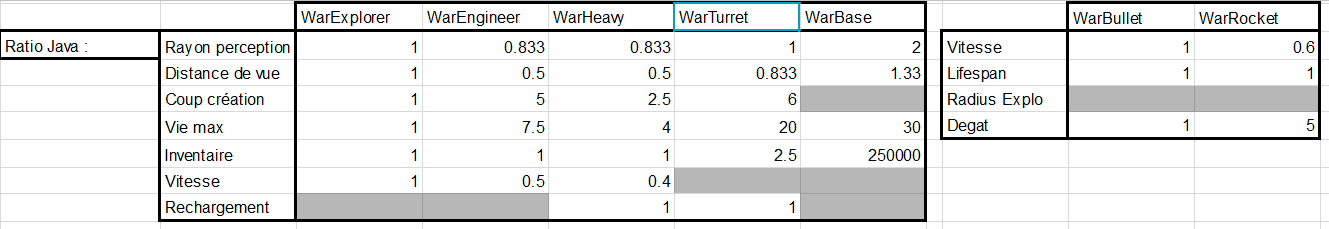
\includegraphics[scale=0.5]{DATA/ratio.png}
\captionof{figure} {Tableau des ratio}
\end{adjustwidth}
\paragraph{}
Nous modifions ensuite les valeurs dans le tableau “valeur par défaut”, ce qui modifie automatiquement les valeurs dans le tableau “calcul via ratio” qui nous sert de référence pour remplir le tableau “Rééquilibrage Unity” dans lequel nous modifions les valeurs à la main pour équilibrer au mieux la version actuelle.

\paragraph{}
\begin{adjustwidth}{-3em}{}
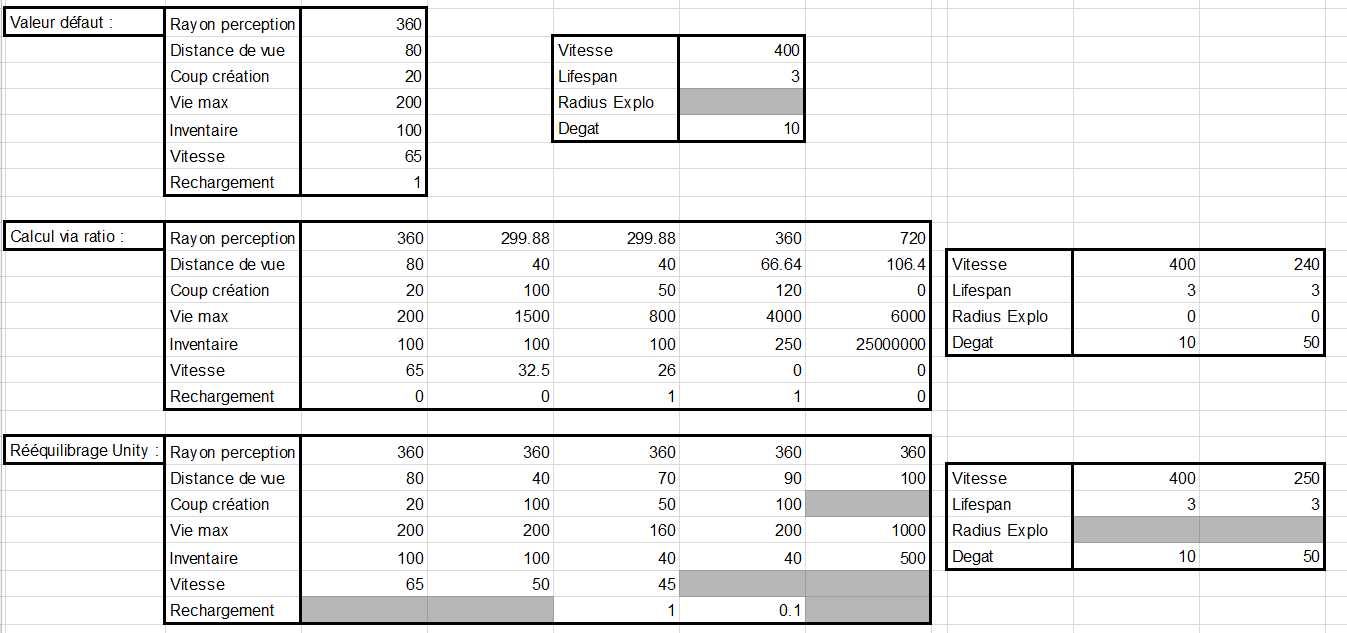
\includegraphics[scale=0.45]{DATA/equilibrage.png}
\captionof{figure} {Calcul des statistiques}
\end{adjustwidth}
\paragraph{}

    La seule unité pour laquelle nous ne calculons pas statistiques est le WarLight. En effet, cette unité s’est vu rajoutée au cours du projet et n’était donc pas présente lors de la création du tableur. Ses caractéristiques sont donc choisies de manière subjective en se basant sur les statistiques des autres unités. Nous souhaitons que cette unité soit un peu plus lente que les explorateurs. Elle doit également être de résistance moyenne, faire peu de dégâts mais avoir une cadence de tir élevée. \newline
Une fois les unités modifiées, des tests avec des équipes adoptant des stratégies différentes sont effectués. Lors de nos test, nous nous somme rendu compte que l’ajout d’une nouvelle unité rendaient l’équilibrage délicat car cela demande de reconsidérer le rôle de toutes les autres unités. Le fait de ne pas disposer de toutes les possibilités disponibles dans la version Java rend également l’équilibrage difficile car nous ne pouvons pas réellement nous servir d’elle comme référence.
\paragraph{}
Tout d’abord, le WarHeavy semblait presque inutile. En effet, la particularité de cette unité dans la version Java était de pouvoir tirer au-delà de son champs de vision. Ses coéquipiers pouvaient lui transmettre des coordonnées. L’unité s’orientait alors dans cette direction et faisait feu sur une cible qu’elle ne distinguait pas. Cependant, cette fonctionnalité n’étant pas présent dans notre version, le WarHeavy possédait des caractéristiques trop faibles pour justifier son coût de création. Le plus gros ennui était sa distance de vue trop petite. En augmentant simplement cette caractéristique, on risquait de créer une unité trop forte qui rendait les WarLight inutiles. \newline
Nous avons donc décidé de réduire l’angle de perception et d’augmenter la portée de son champs de vision. Ainsi, les WarHeavy détectent mieux les ennemis mais sont plus vulnérables aux attaques qui arrivent de côté.
\paragraph{}
Les autres réglages ont plus été des règlements mineurs sur les autres unités pour obtenir des parties plus dynamique. On a par exemple légèrement augmenté les dégâts des unités offensives pour que les parties se terminent plus rapidement.


\newpage
\part{L'avenir du projet}
\chapter{Amélioration possible}

% Uncomment the following two lines if you want to have a bibliography
%\bibliographystyle{alpha}
%\bibliography{document}

\end{document}





